\documentclass[letterpaper,11pt]{report}
\usepackage[top=1.0in,bottom=1.0in,left=0.1in,right=0.1in]{geometry}
\usepackage{verbatim}
\usepackage{amssymb}
\usepackage{graphicx}
\usepackage{longtable}
\usepackage{amsfonts}
\usepackage{amsmath}
\usepackage{hyperref}
\usepackage{float}
\usepackage{setspace}
\usepackage[acronym,toc]{glossaries}  % acronyms inclusion
\usepackage{color,soul}
\makeglossary
\include{acros}
\usepackage{gensymb}
\usepackage{amssymb}
\usepackage{enumitem}
\usepackage{csquotes}
\usepackage{subcaption}
\usepackage{tikz}
\usetikzlibrary{positioning, arrows, decorations, shapes}
\usetikzlibrary{shapes.geometric,arrows}

\definecolor{illiniblue}{HTML}{B1C6E2}
\definecolor{illiniorange}{HTML}{f8c2a2}
\definecolor{pink}{HTML}{e2b1c2}
\definecolor{green}{HTML}{c2e2b1}
\definecolor{purple}{HTML}{b9b1e2}
\tikzstyle{snoblock} = [rectangle, 
text width=5em, text centered,  minimum height=0em]
\tikzstyle{noblock} = [rectangle, 
text width=5em, text centered,  minimum height=3em]
\tikzstyle{loblock} = [rectangle, draw, fill=illiniorange, 
text width=15em, text centered, rounded corners, minimum height=3em]
\tikzstyle{lbblock} = [rectangle, draw, fill=illiniblue, 
text width=15em, text centered, rounded corners, minimum height=3em]
\tikzstyle{oblock} = [rectangle, draw, fill=illiniorange, 
text width=10em, text centered, rounded corners, minimum height=3em]
\tikzstyle{bblock} = [rectangle, draw, fill=illiniblue, 
text width=10em, text centered, rounded corners, minimum height=3em]
\tikzstyle{arrow} = [thick,->,>=stealth]
\tikzstyle{pblock} = [rectangle, draw, fill=pink, 
text width=10em, text centered, rounded corners, minimum height=3em]
\tikzstyle{gblock} = [rectangle, draw, fill=green, 
text width=10em, text centered, rounded corners, minimum height=3em]
\tikzstyle{ppblock} = [rectangle, draw, fill=purple, 
text width=10em, text centered, rounded corners, minimum height=3em]
\tikzstyle{lppblock} = [rectangle, draw, fill=purple, 
text width=15em, text centered, rounded corners, minimum height=3em]
\tikzstyle{arrow} = [thick,->,>=stealth]
\tikzstyle{bbblock} = [rectangle, draw, fill=illiniblue, 
text width=1em, text centered, rounded corners, minimum height=1em]
\tikzstyle{boblock} = [rectangle, draw, fill=illiniorange, 
text width=1em, text centered, rounded corners, minimum height=1em]
\tikzstyle{bpblock} = [rectangle, draw, fill=pink, 
text width=1em, text centered, rounded corners, minimum height=1em]
\tikzstyle{bgblock} = [rectangle, draw, fill=green, 
text width=1em, text centered, rounded corners, minimum height=1em]
\tikzstyle{bppblock} = [rectangle, draw, fill=purple, 
text width=1em, text centered, rounded corners, minimum height=1em]
\renewcommand{\thesection}{\arabic{section}}

\author{Gwendolyn J.Y. Chee, Kathryn D. Huff}

\title{FHR Benchmark Optional Figures }
\begin{document}
\maketitle

\section{Fission source distribution (c)}
\begin{figure}[H]
    \centering
    \begin{subfigure}{.33\textwidth}
        \centering
        \includegraphics[width=\linewidth]{../../phase1a/case1a/analysis_output/p1a_1a_c.png}
        \caption{}
      \end{subfigure}%
      \begin{subfigure}{.33\textwidth}
        \centering
        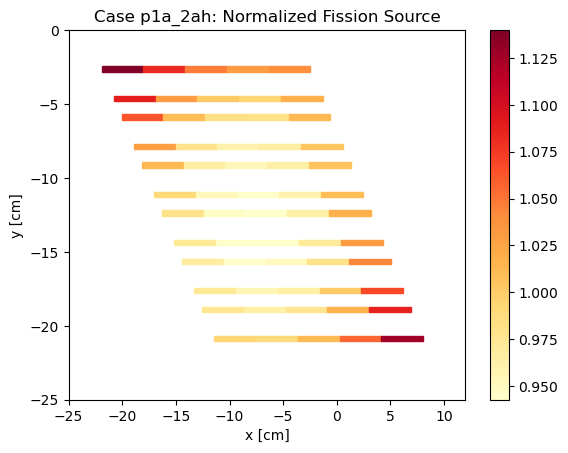
\includegraphics[width=\linewidth]{../../phase1a/case2ah/analysis_output/p1a_2ah_c.png}
        \caption{}
      \end{subfigure}
      \begin{subfigure}{.33\textwidth}
        \centering
        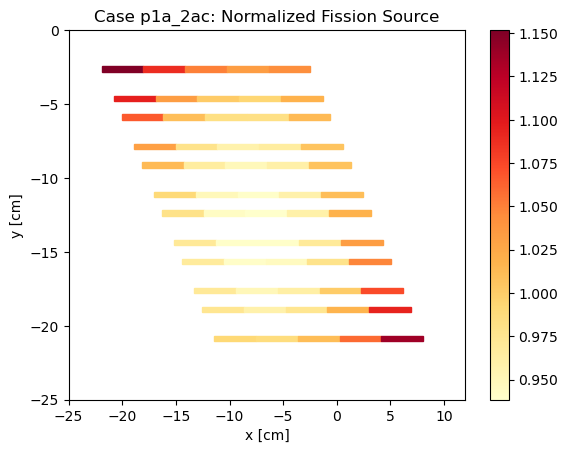
\includegraphics[width=\linewidth]{../../phase1a/case2ac/analysis_output/p1a_2ac_c.png}
        \caption{}
      \end{subfigure}
      \begin{subfigure}{.33\textwidth}
        \centering
        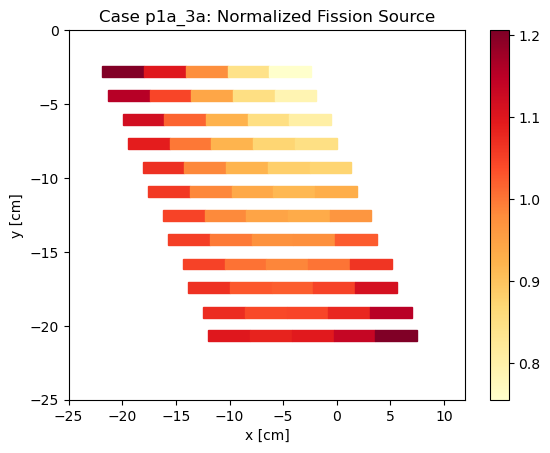
\includegraphics[width=\linewidth]{../../phase1a/case3a/analysis_output/p1a_3a_c.png}
        \caption{}
      \end{subfigure}
      \begin{subfigure}{.33\textwidth}
        \centering
        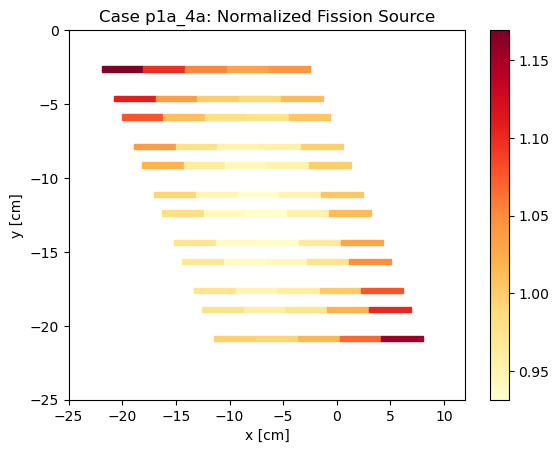
\includegraphics[width=\linewidth]{../../phase1a/case4a/analysis_output/p1a_4a_c.png}
        \caption{}
      \end{subfigure}
      \begin{subfigure}{.32\textwidth}
        \centering
        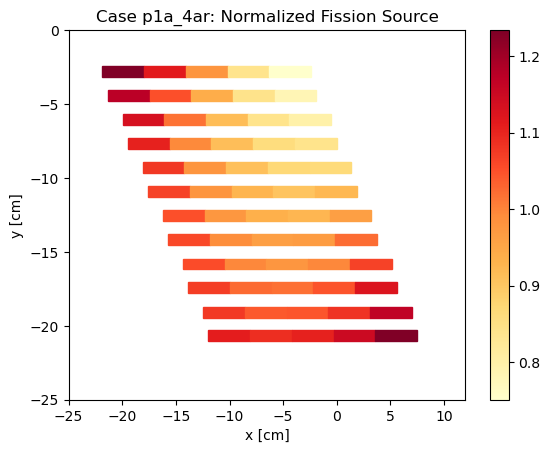
\includegraphics[width=\linewidth]{../../phase1a/case4ar/analysis_output/p1a_4ar_c.png}
        \caption{}
      \end{subfigure}
      \begin{subfigure}{.33\textwidth}
        \centering
        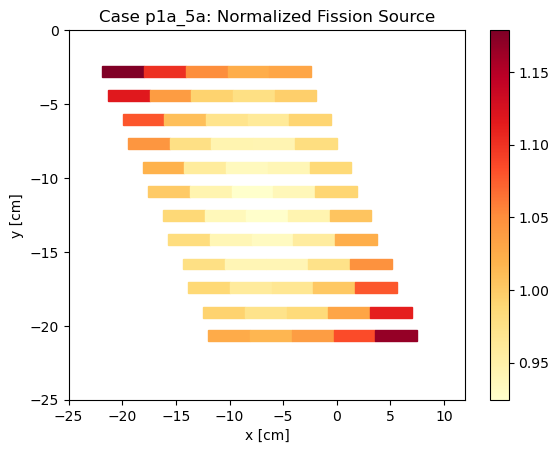
\includegraphics[width=\linewidth]{../../phase1a/case5a/analysis_output/p1a_5a_c.png}
        \caption{}
      \end{subfigure}
      \begin{subfigure}{.33\textwidth}
        \centering
        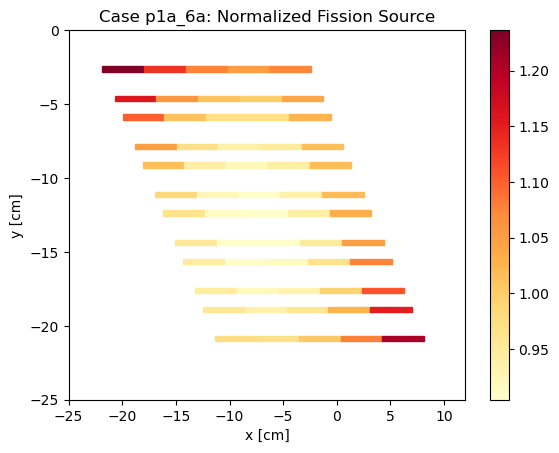
\includegraphics[width=\linewidth]{../../phase1a/case6a/analysis_output/p1a_6a_c.png}
        \caption{}
      \end{subfigure}
      \begin{subfigure}{.32\textwidth}
        \centering
        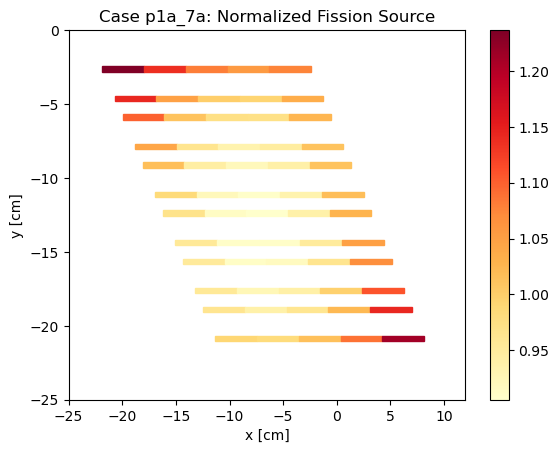
\includegraphics[width=\linewidth]{../../phase1a/case7a/analysis_output/p1a_7a_c.png}
        \caption{}
      \end{subfigure}
    \caption{}
    \label{fig:test}
    \end{figure}

\pagebreak 

\section{Visualized distribution of neutron flux by 1/5-th stripe in 3 coarse energy groups (e)}
\begin{figure}[H]
    \centering
    \begin{subfigure}{.33\textwidth}
        \centering
        \includegraphics[width=1.1\linewidth]{../../phase1a/case1a/analysis_output/p1a_1a_e_eg1.png}
        \caption{}
      \end{subfigure}%
      \begin{subfigure}{.33\textwidth}
        \centering
        \includegraphics[width=1.1\linewidth]{../../phase1a/case1a/analysis_output/p1a_1a_e_eg2.png}
        \caption{}
      \end{subfigure}
      \begin{subfigure}{.33\textwidth}
        \centering
        \includegraphics[width=1.1\linewidth]{../../phase1a/case1a/analysis_output/p1a_1a_e_eg3.png}
        \caption{}
      \end{subfigure}

      \begin{subfigure}{.33\textwidth}
        \centering
        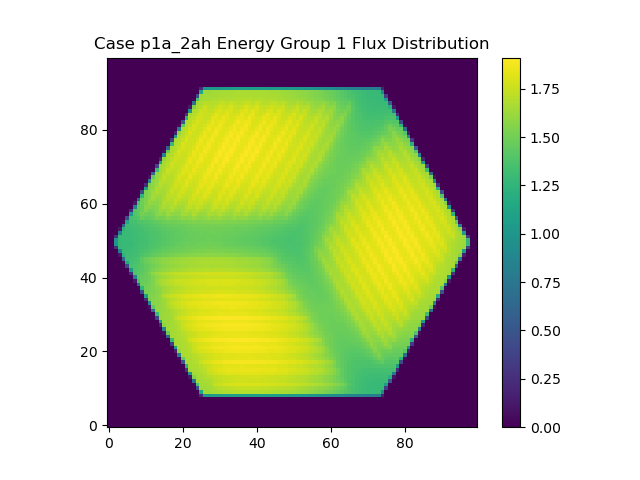
\includegraphics[width=1.1\linewidth]{../../phase1a/case2ah/analysis_output/p1a_2ah_e_eg1.png}
        \caption{}
      \end{subfigure}%
      \begin{subfigure}{.33\textwidth}
        \centering
        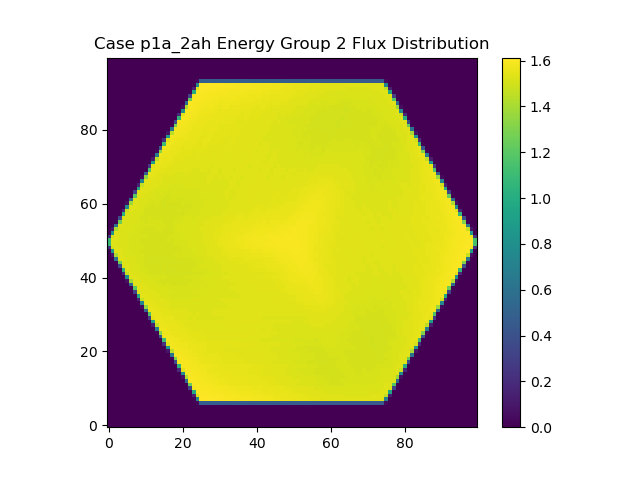
\includegraphics[width=1.1\linewidth]{../../phase1a/case2ah/analysis_output/p1a_2ah_e_eg2.png}
        \caption{}
      \end{subfigure}
      \begin{subfigure}{.33\textwidth}
        \centering
        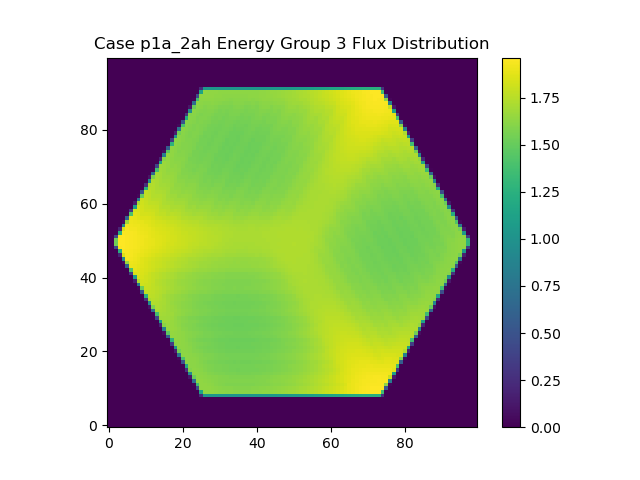
\includegraphics[width=1.1\linewidth]{../../phase1a/case2ah/analysis_output/p1a_2ah_e_eg3.png}
        \caption{}
      \end{subfigure}

      \begin{subfigure}{.33\textwidth}
        \centering
        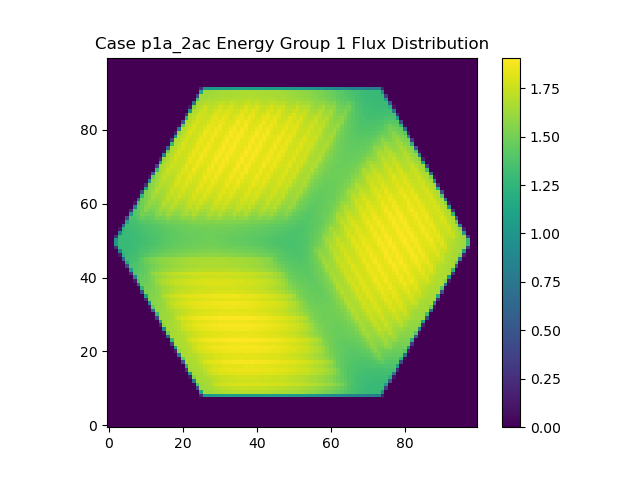
\includegraphics[width=1.1\linewidth]{../../phase1a/case2ac/analysis_output/p1a_2ac_e_eg1.png}
        \caption{}
      \end{subfigure}%
      \begin{subfigure}{.33\textwidth}
        \centering
        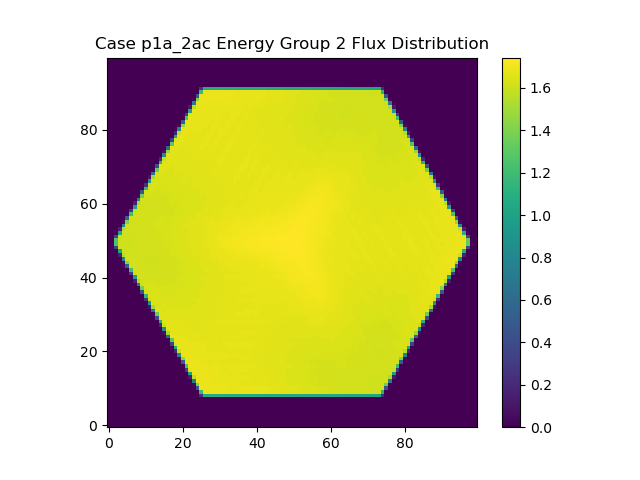
\includegraphics[width=1.1\linewidth]{../../phase1a/case2ac/analysis_output/p1a_2ac_e_eg2.png}
        \caption{}
      \end{subfigure}
      \begin{subfigure}{.33\textwidth}
        \centering
        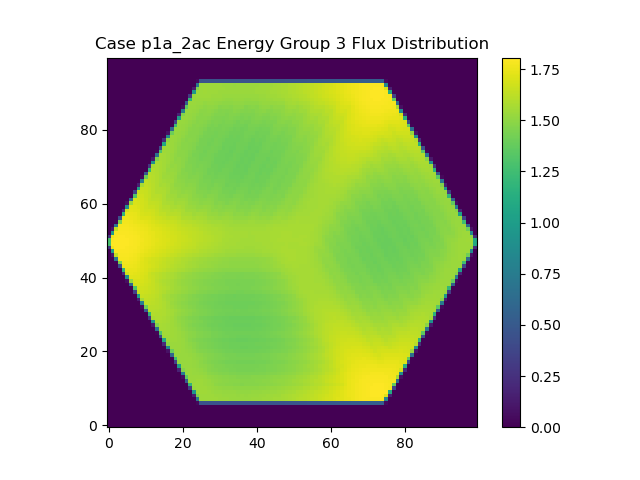
\includegraphics[width=1.1\linewidth]{../../phase1a/case2ac/analysis_output/p1a_2ac_e_eg3.png}
        \caption{}
      \end{subfigure}
    \caption{}
    \label{fig:test}
    \end{figure}

    \begin{figure}[H]
        \centering
          \begin{subfigure}{.33\textwidth}
            \centering
            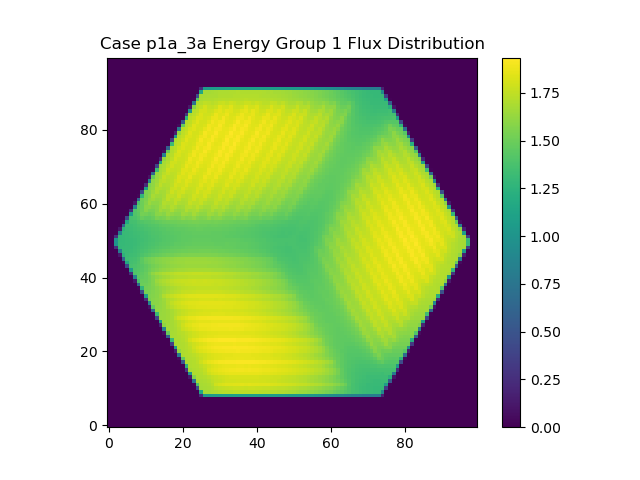
\includegraphics[width=1.1\linewidth]{../../phase1a/case3a/analysis_output/p1a_3a_e_eg1.png}
            \caption{}
          \end{subfigure}%
          \begin{subfigure}{.33\textwidth}
            \centering
            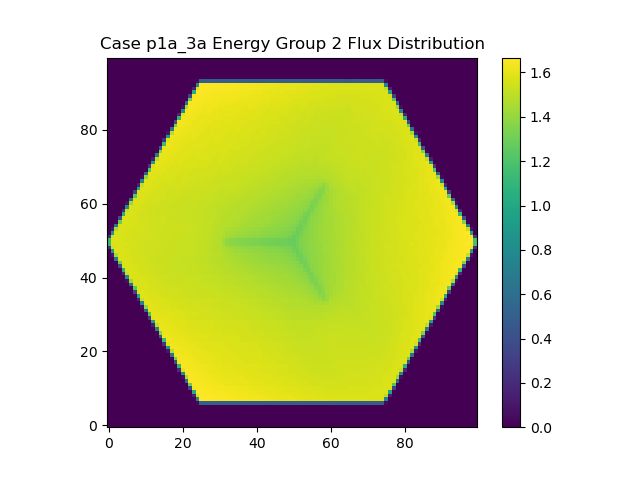
\includegraphics[width=1.1\linewidth]{../../phase1a/case3a/analysis_output/p1a_3a_e_eg2.png}
            \caption{}
          \end{subfigure}
          \begin{subfigure}{.33\textwidth}
            \centering
            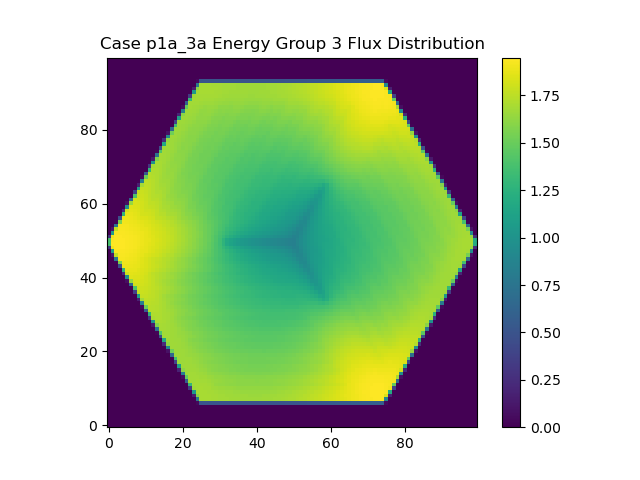
\includegraphics[width=1.1\linewidth]{../../phase1a/case3a/analysis_output/p1a_3a_e_eg3.png}
            \caption{}
          \end{subfigure}

          \begin{subfigure}{.33\textwidth}
            \centering
            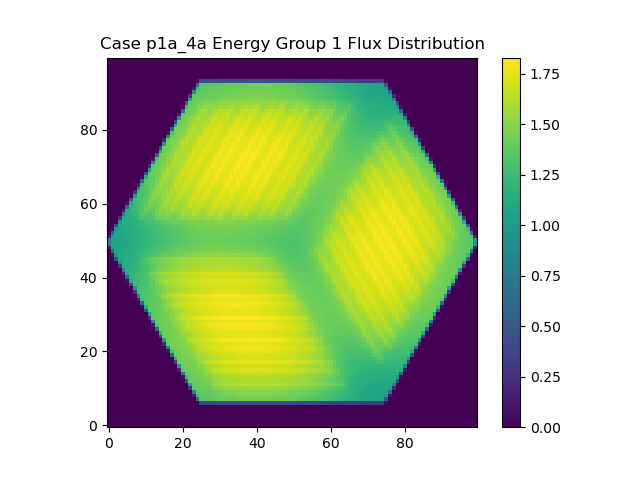
\includegraphics[width=1.1\linewidth]{../../phase1a/case4a/analysis_output/p1a_4a_e_eg1.png}
            \caption{}
          \end{subfigure}%
          \begin{subfigure}{.33\textwidth}
            \centering
            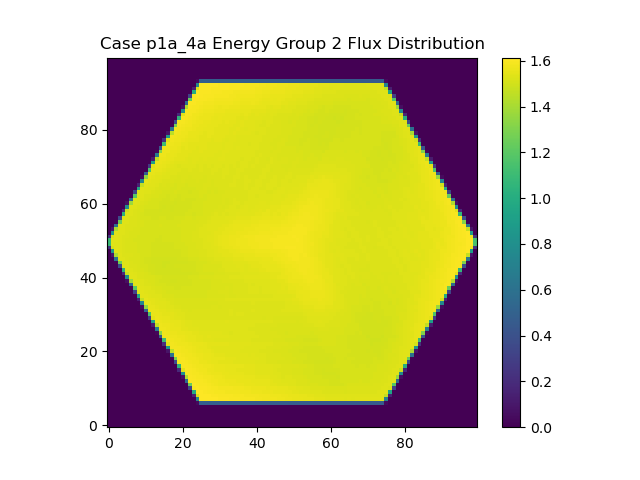
\includegraphics[width=1.1\linewidth]{../../phase1a/case4a/analysis_output/p1a_4a_e_eg2.png}
            \caption{}
          \end{subfigure}
          \begin{subfigure}{.33\textwidth}
            \centering
            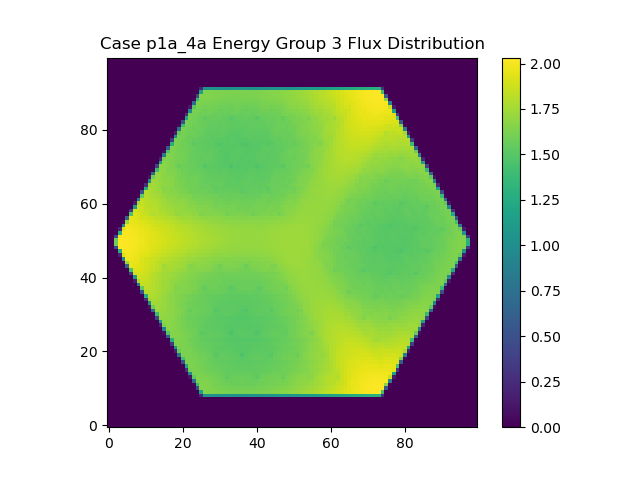
\includegraphics[width=1.1\linewidth]{../../phase1a/case4a/analysis_output/p1a_4a_e_eg3.png}
            \caption{}
          \end{subfigure}

          \begin{subfigure}{.33\textwidth}
            \centering
            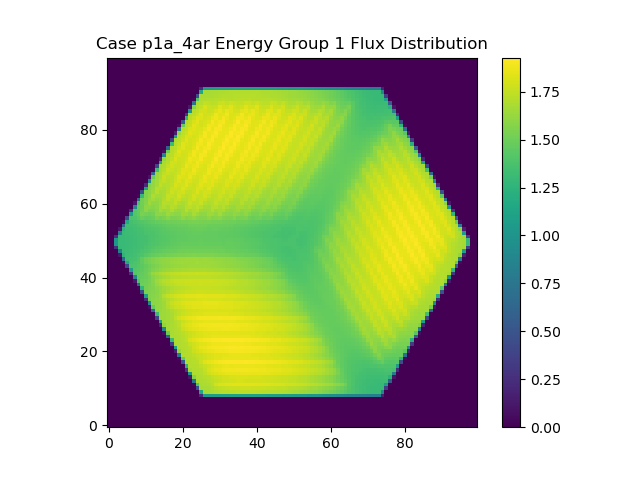
\includegraphics[width=1.1\linewidth]{../../phase1a/case4ar/analysis_output/p1a_4ar_e_eg1.png}
            \caption{}
          \end{subfigure}%
          \begin{subfigure}{.33\textwidth}
            \centering
            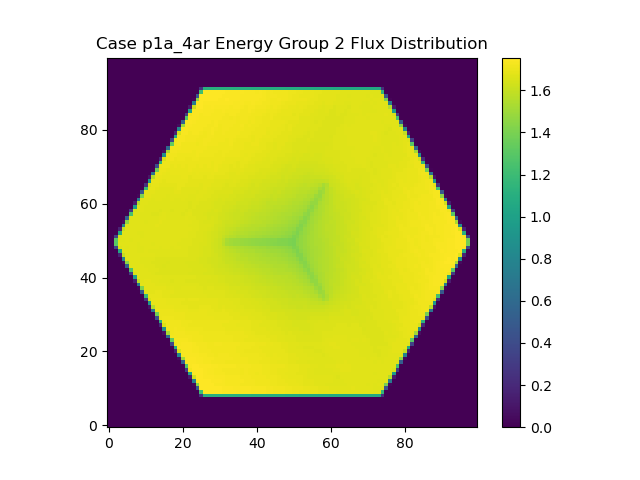
\includegraphics[width=1.1\linewidth]{../../phase1a/case4ar/analysis_output/p1a_4ar_e_eg2.png}
            \caption{}
          \end{subfigure}
          \begin{subfigure}{.33\textwidth}
            \centering
            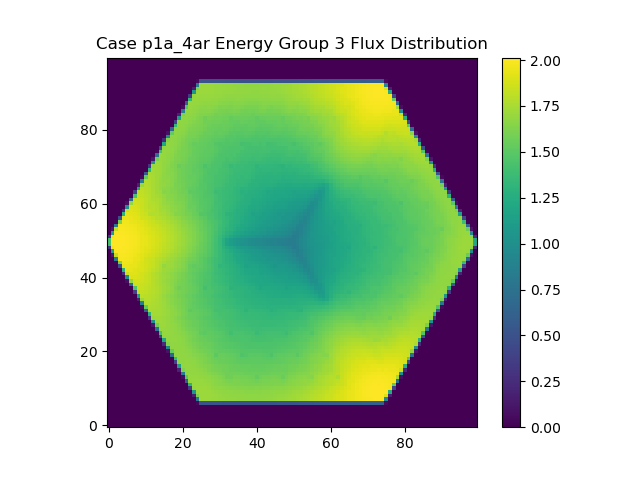
\includegraphics[width=1.1\linewidth]{../../phase1a/case4ar/analysis_output/p1a_4ar_e_eg3.png}
            \caption{}
          \end{subfigure}
        \caption{}
        \label{fig:test}
        \end{figure}

        \begin{figure}[H]
          \centering
            \begin{subfigure}{.33\textwidth}
              \centering
              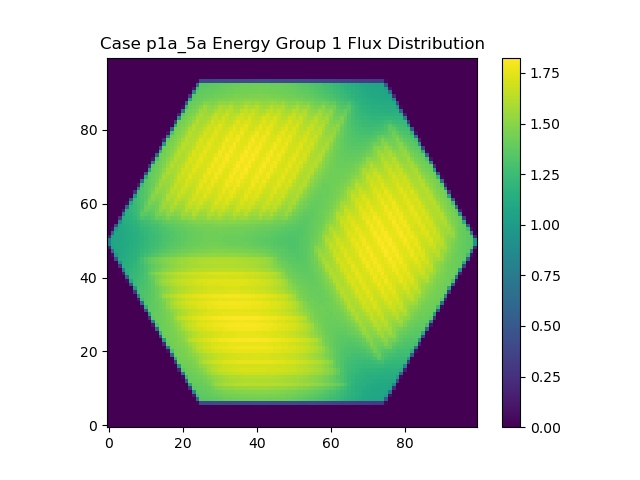
\includegraphics[width=1.1\linewidth]{../../phase1a/case5a/analysis_output/p1a_5a_e_eg1.png}
              \caption{}
            \end{subfigure}%
            \begin{subfigure}{.33\textwidth}
              \centering
              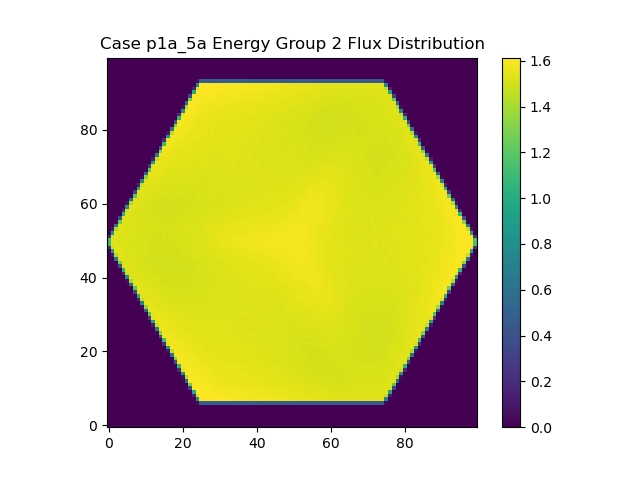
\includegraphics[width=1.1\linewidth]{../../phase1a/case5a/analysis_output/p1a_5a_e_eg2.png}
              \caption{}
            \end{subfigure}
            \begin{subfigure}{.33\textwidth}
              \centering
              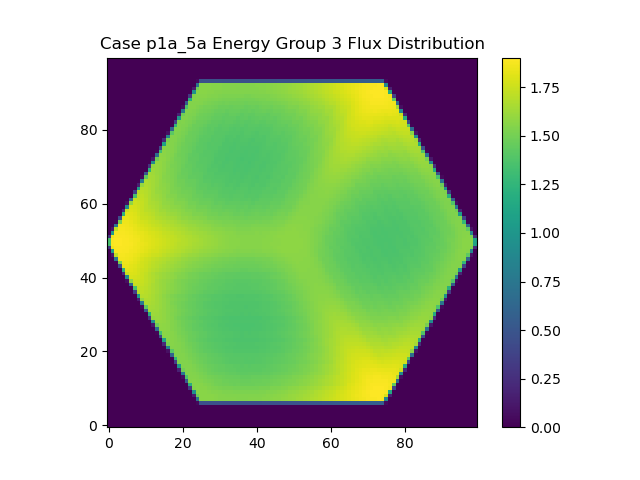
\includegraphics[width=1.1\linewidth]{../../phase1a/case5a/analysis_output/p1a_5a_e_eg3.png}
              \caption{}
            \end{subfigure}
  
            \begin{subfigure}{.33\textwidth}
              \centering
              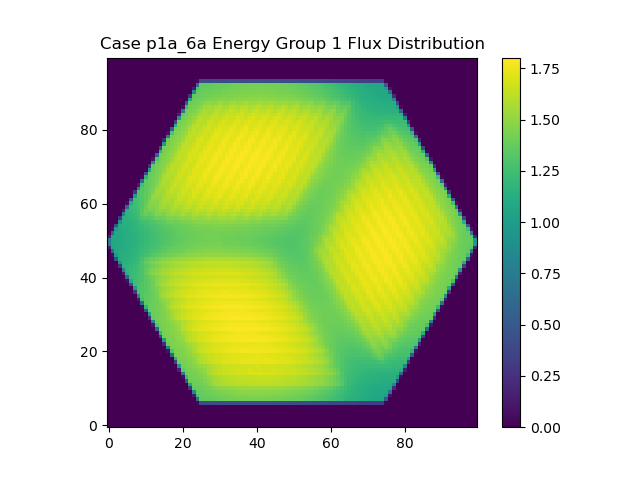
\includegraphics[width=1.1\linewidth]{../../phase1a/case6a/analysis_output/p1a_6a_e_eg1.png}
              \caption{}
            \end{subfigure}%
            \begin{subfigure}{.33\textwidth}
              \centering
              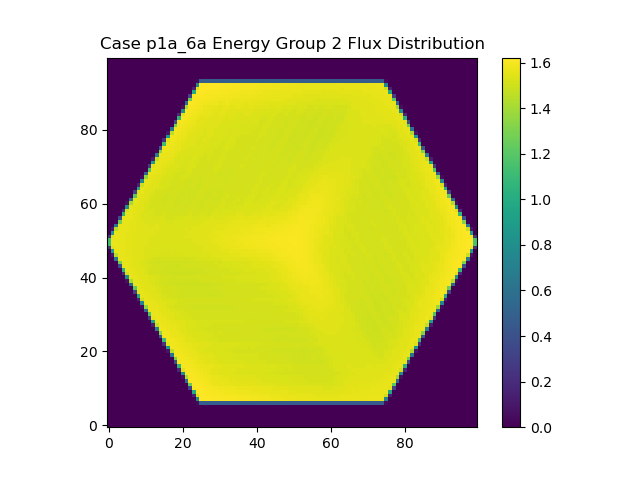
\includegraphics[width=1.1\linewidth]{../../phase1a/case6a/analysis_output/p1a_6a_e_eg2.png}
              \caption{}
            \end{subfigure}
            \begin{subfigure}{.33\textwidth}
              \centering
              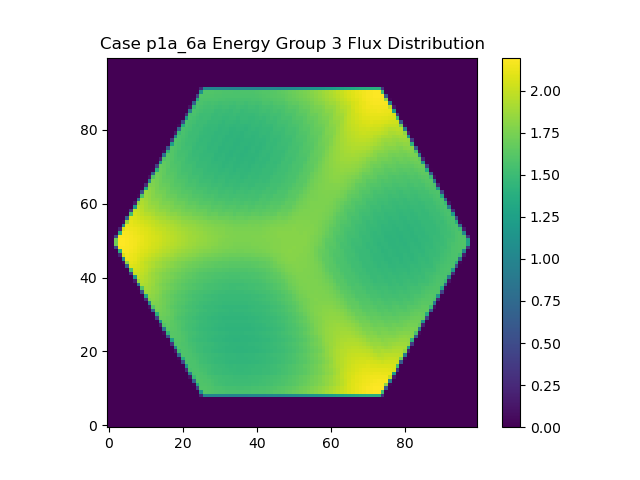
\includegraphics[width=1.1\linewidth]{../../phase1a/case6a/analysis_output/p1a_6a_e_eg3.png}
              \caption{}
            \end{subfigure}
  
            \begin{subfigure}{.33\textwidth}
              \centering
              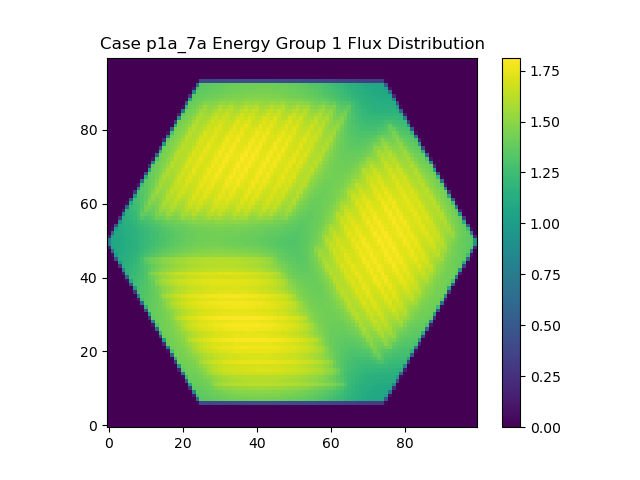
\includegraphics[width=1.1\linewidth]{../../phase1a/case7a/analysis_output/p1a_7a_e_eg1.png}
              \caption{}
            \end{subfigure}%
            \begin{subfigure}{.33\textwidth}
              \centering
              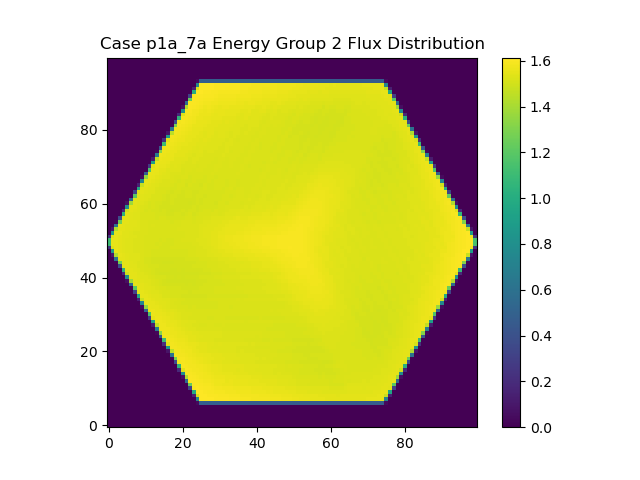
\includegraphics[width=1.1\linewidth]{../../phase1a/case7a/analysis_output/p1a_7a_e_eg2.png}
              \caption{}
            \end{subfigure}
            \begin{subfigure}{.33\textwidth}
              \centering
              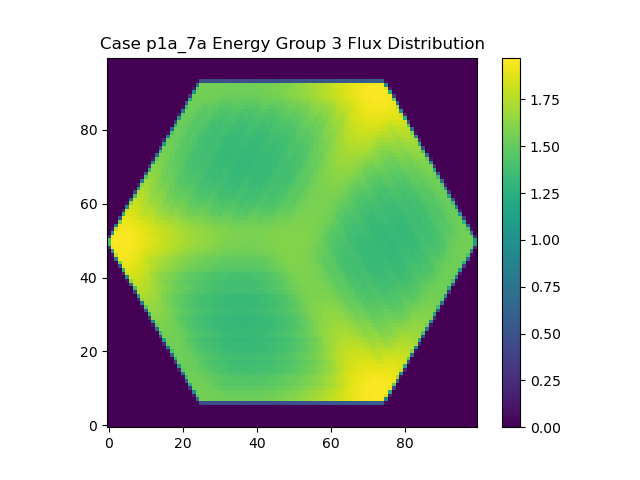
\includegraphics[width=1.1\linewidth]{../../phase1a/case7a/analysis_output/p1a_7a_e_eg3.png}
              \caption{}
            \end{subfigure}
          \caption{}
          \label{fig:test}
          \end{figure}

\section{Neutron spectrum, fuel assembly average (f)}
        \begin{figure}[H]
            \centering
            \begin{subfigure}{.33\textwidth}
                \centering
                \includegraphics[width=\linewidth]{../../phase1a/case1a/analysis_output/p1a_1a_f.png}
                \caption{}
              \end{subfigure}%
              \begin{subfigure}{.33\textwidth}
                \centering
                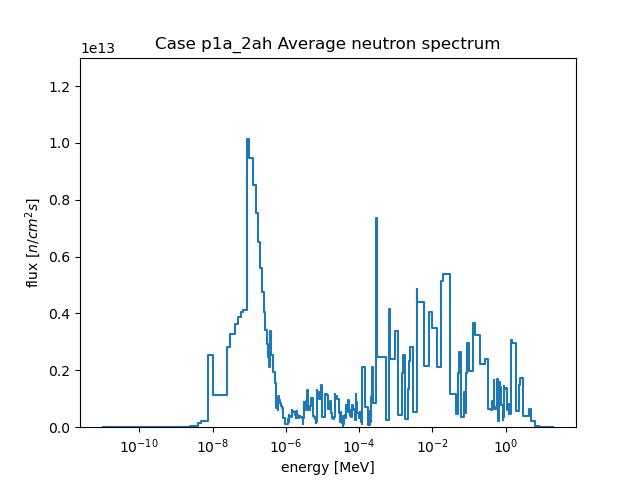
\includegraphics[width=\linewidth]{../../phase1a/case2ah/analysis_output/p1a_2ah_f.png}
                \caption{}
              \end{subfigure}
              \begin{subfigure}{.33\textwidth}
                \centering
                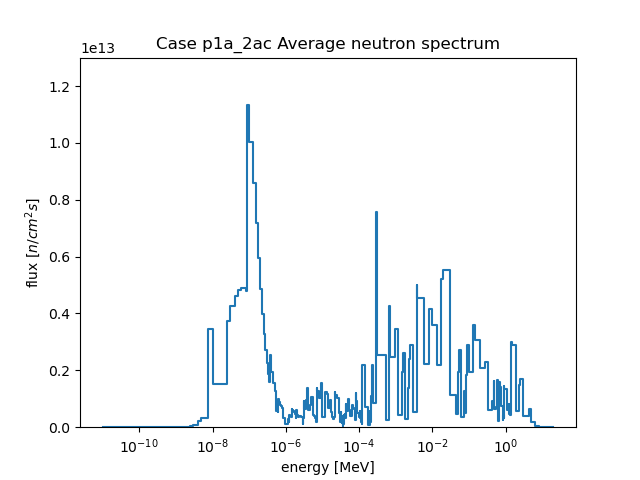
\includegraphics[width=\linewidth]{../../phase1a/case2ac/analysis_output/p1a_2ac_f.png}
                \caption{}
              \end{subfigure}
              \begin{subfigure}{.33\textwidth}
                \centering
                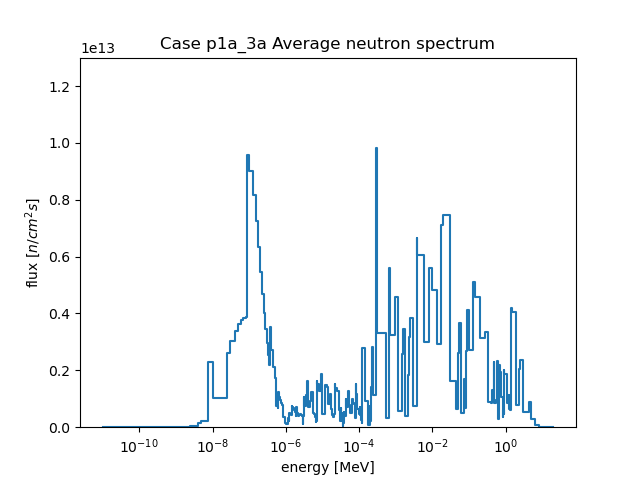
\includegraphics[width=\linewidth]{../../phase1a/case3a/analysis_output/p1a_3a_f.png}
                \caption{}
              \end{subfigure}
              \begin{subfigure}{.33\textwidth}
                \centering
                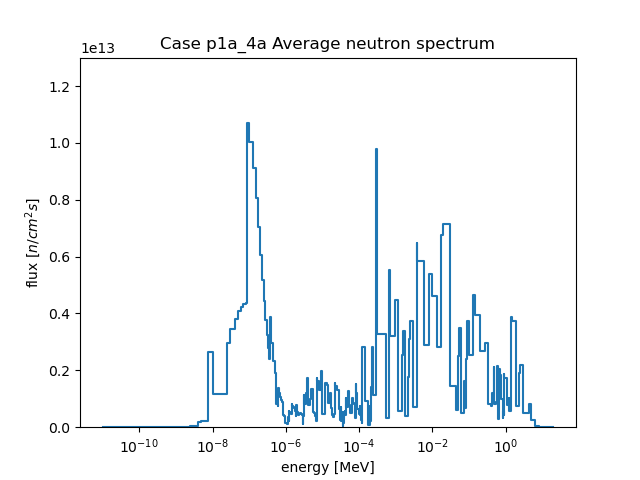
\includegraphics[width=\linewidth]{../../phase1a/case4a/analysis_output/p1a_4a_f.png}
                \caption{}
              \end{subfigure}
              \begin{subfigure}{.32\textwidth}
                \centering
                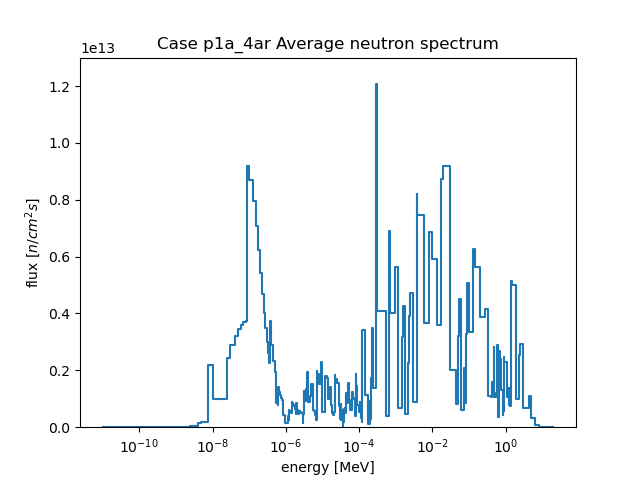
\includegraphics[width=\linewidth]{../../phase1a/case4ar/analysis_output/p1a_4ar_f.png}
                \caption{}
              \end{subfigure}
              \begin{subfigure}{.33\textwidth}
                \centering
                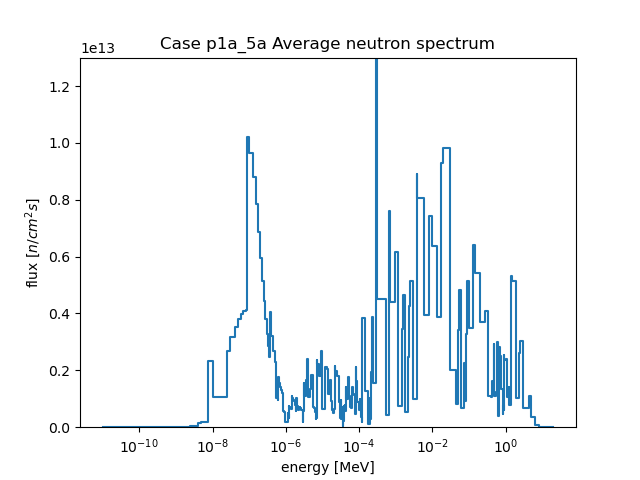
\includegraphics[width=\linewidth]{../../phase1a/case5a/analysis_output/p1a_5a_f.png}
                \caption{}
              \end{subfigure}
              \begin{subfigure}{.33\textwidth}
                \centering
                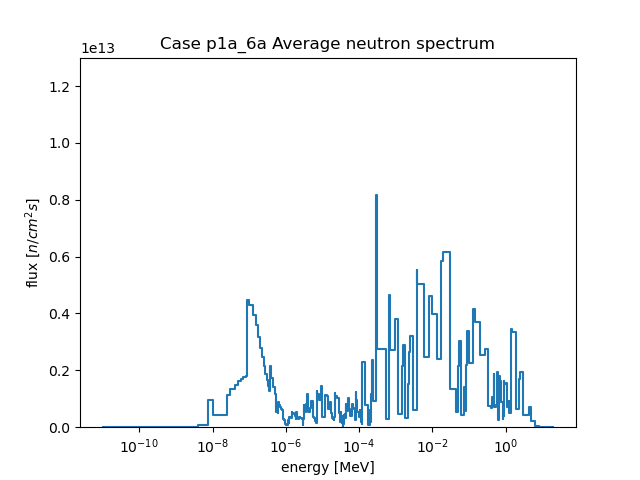
\includegraphics[width=\linewidth]{../../phase1a/case6a/analysis_output/p1a_6a_f.png}
                \caption{}
              \end{subfigure}
              \begin{subfigure}{.32\textwidth}
                \centering
                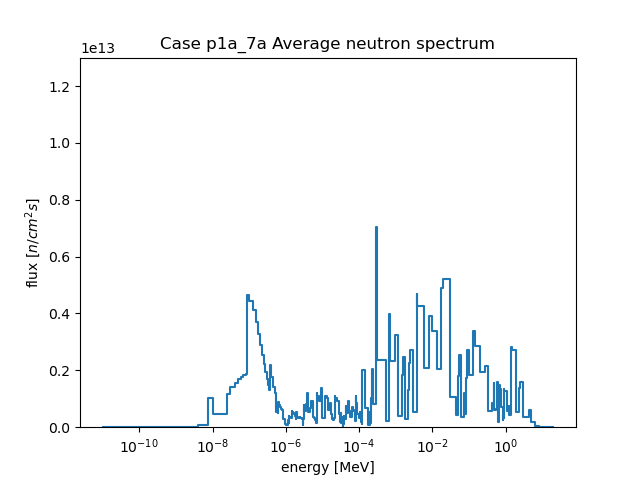
\includegraphics[width=\linewidth]{../../phase1a/case7a/analysis_output/p1a_7a_f.png}
                \caption{}
              \end{subfigure}
            \caption{}
            \label{fig:test}
            \end{figure}

\end{document}
